\section{Methodology}
\label{sec:methodology}

This section details the methodology employed in this study. We introduce a novel framework that leverages multiple modalities for the development of atmospheric visibility estimation solutions. A key component of this work is the construction of a new dataset, SeeSet V1, which encompasses both ground-level and elevated altitude conditions, addressing a critical gap in existing resources.

\subsection{SeeSet V1 Dataset}
\label{sec:seeset}

To address the limitations of existing datasets and to encompass a broader range of real-world operational scenarios, we have developed a novel aerial imagery dataset designated SeeSet V1. This dataset has been meticulously curated to include dynamic views from multiple locations, capturing scenery from both ground-based and aerial perspectives.

This section provides a comprehensive description of the data collection and labeling procedures (\cref{data_collection}). In \cref{modalities}, we detail the techniques utilized to generate the supplementary image modalities.

\subsubsection{Dataset Collection Process}
\label{data_collection}

The generation of our synthetic dataset was accomplished using an FAA-approved flight simulator. The use of this advanced simulator enabled the systematic and controlled acquisition of images, showcasing a diverse range of viewpoints and visibility degradation levels. The data collection process, as depicted in Figure~\ref{fig:data_collection_process}, commenced at ground level. Visibility was incrementally increased in discrete steps, up to a maximum of 100 miles. Upon reaching this limit, the viewpoint's altitude was elevated, and the visibility was reset to zero. This iterative procedure was continued up to a maximum altitude of 2,000 feet Above Ground Level (AGL).


\begin{figure}[htbp]
\centerline{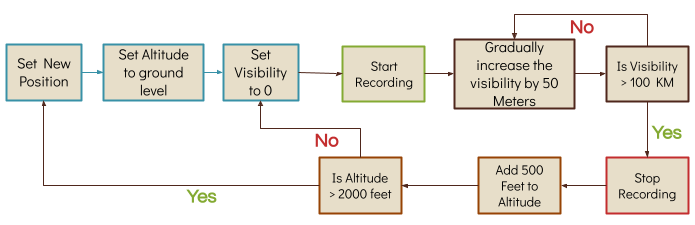
\includegraphics[width=250pt]{imgs/data_collection_pipeline.png}}
\caption{Automatic Dataset Collection Process using X-Plane 11}
\label{fig:data_collection_process}
\end{figure}
 

The collected images are automatically labeled into five discrete bins, each tailored to specific \href{https://www.faa.gov/air_traffic/publications/atpubs/aim_html/}{FAA requirements}. This categorization is based on visibility conditions and regulations relevant to both ground-based and aerial environments. The designated bins serve as the basis for the five labels utilized in training our DL models. 
We report the classes (bins) specifications and the corresponding counts in \cref{tab:vis_img_count}.


\begin{figure}
  \centering
  \begin{subfigure}[b]{0.15\textwidth}
    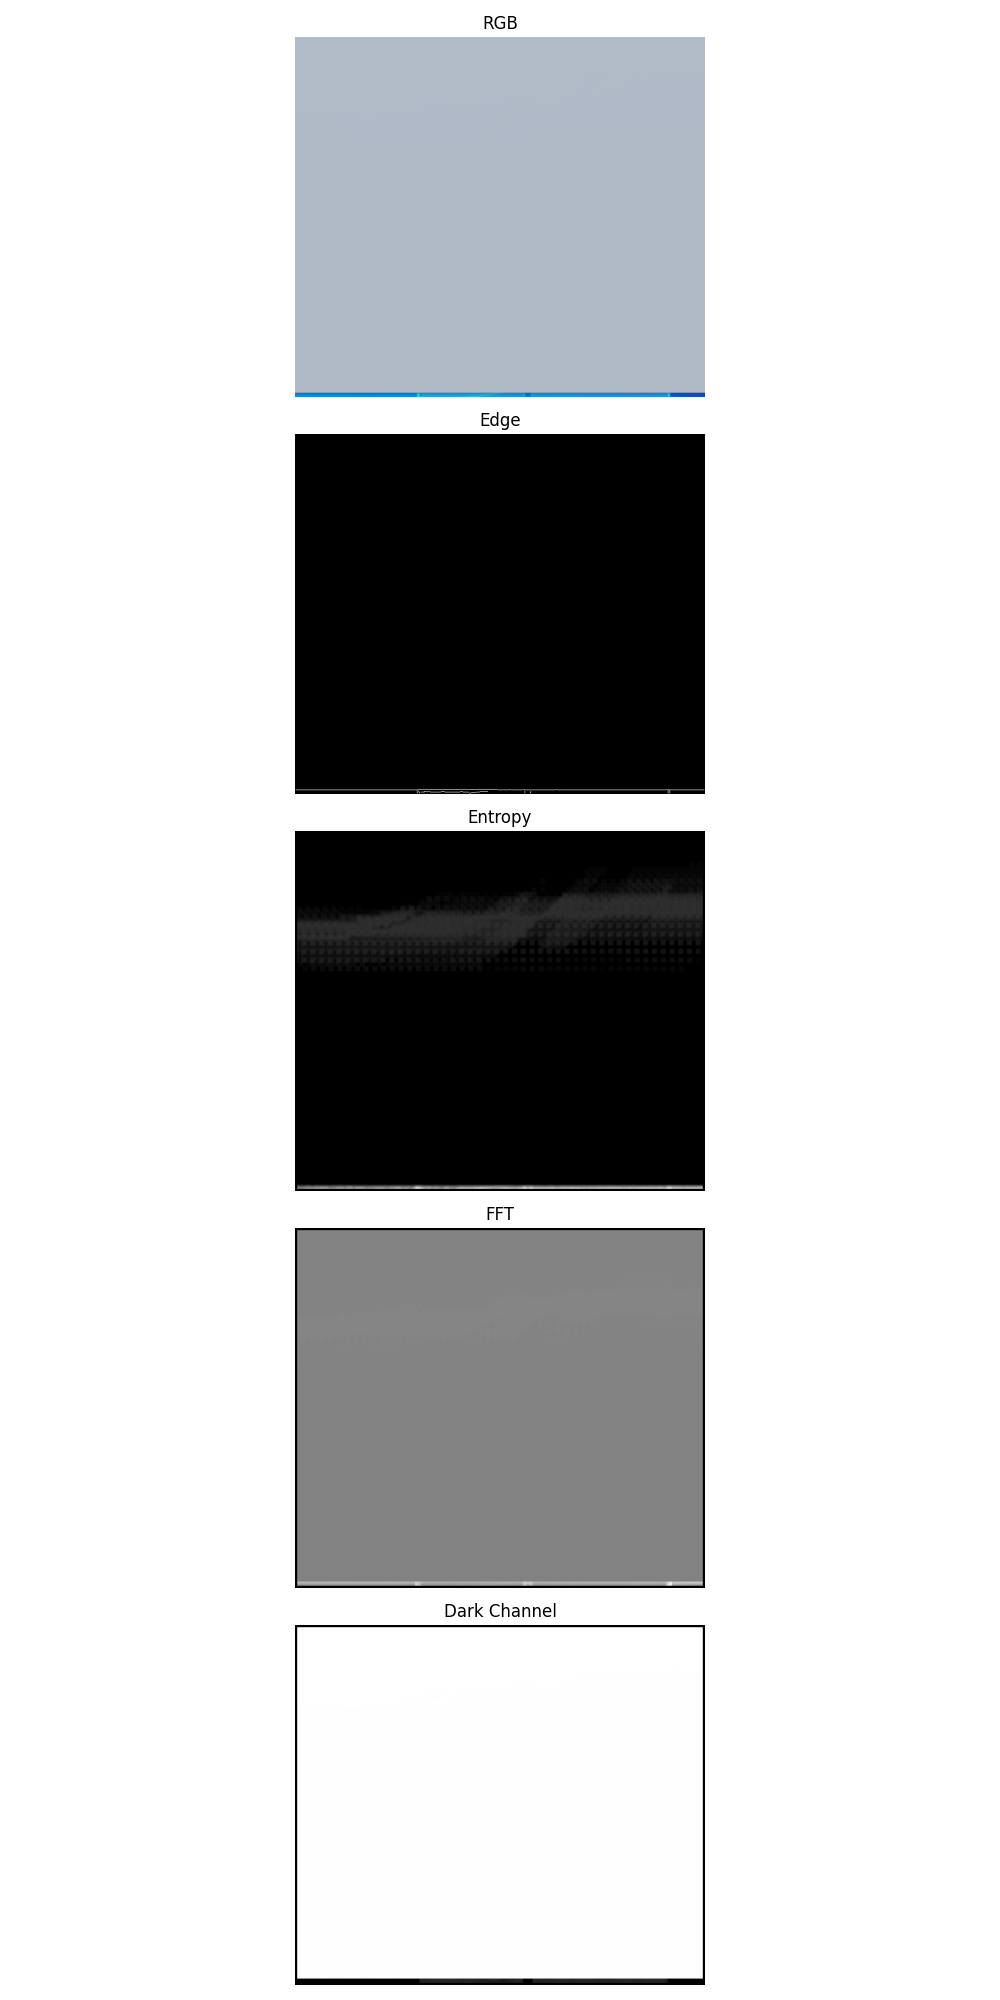
\includegraphics[width=\textwidth, trim={7.5cm 0cm 7.5cm 0cm},clip]{imgs/examples/exp_0_featuresMiles_0.12427454732996136_featuresM_200_features.png}
    \caption{< 0.5 mile}
    \label{subfig:bin0}
  \end{subfigure}
  \begin{subfigure}[b]{0.15\textwidth}
    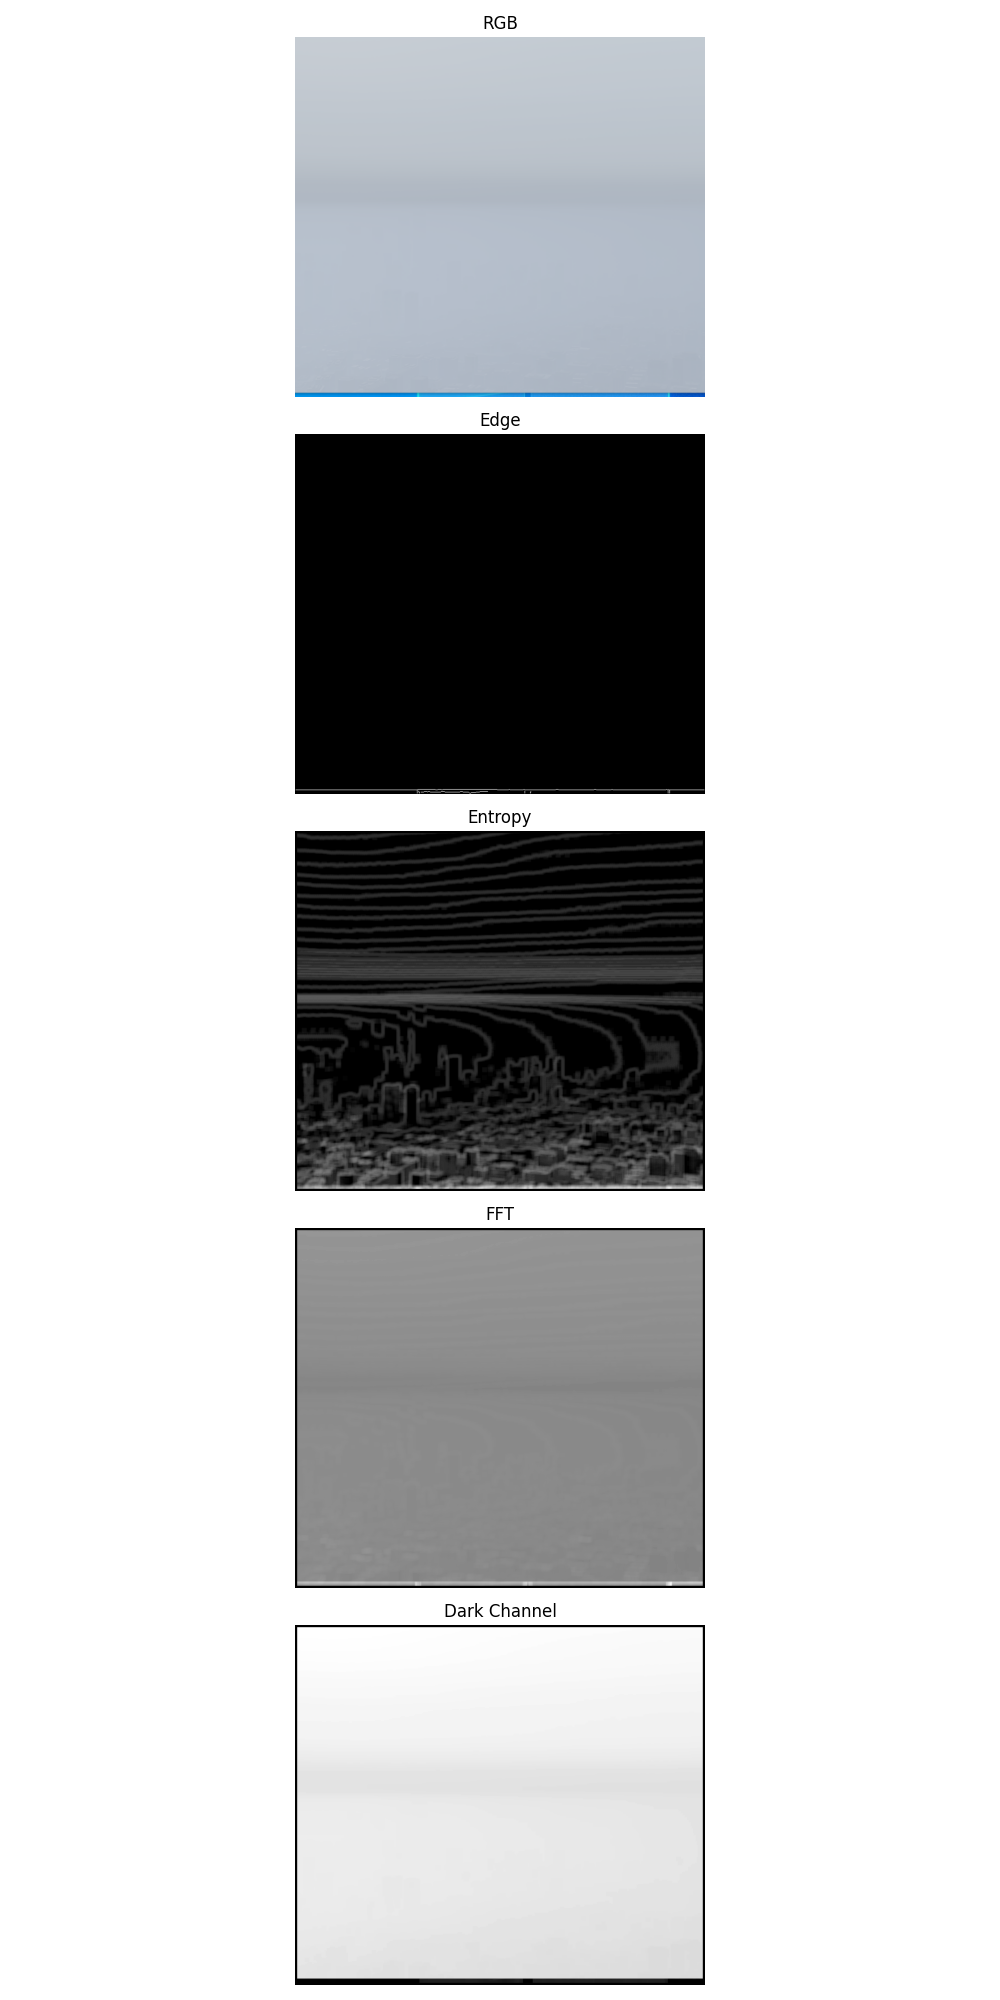
\includegraphics[width=\textwidth, trim={7.5cm 0 7.5cm 0},clip]{imgs/examples/exp_0_featuresMiles_0.9320591049747102_featuresM_1500_features.png}
    \caption{(0.5, 1] miles}
    \label{subfig:bin1}
  \end{subfigure}
  % Add the subfigrow environment here
    \begin{subfigure}[b]{0.15\textwidth}
      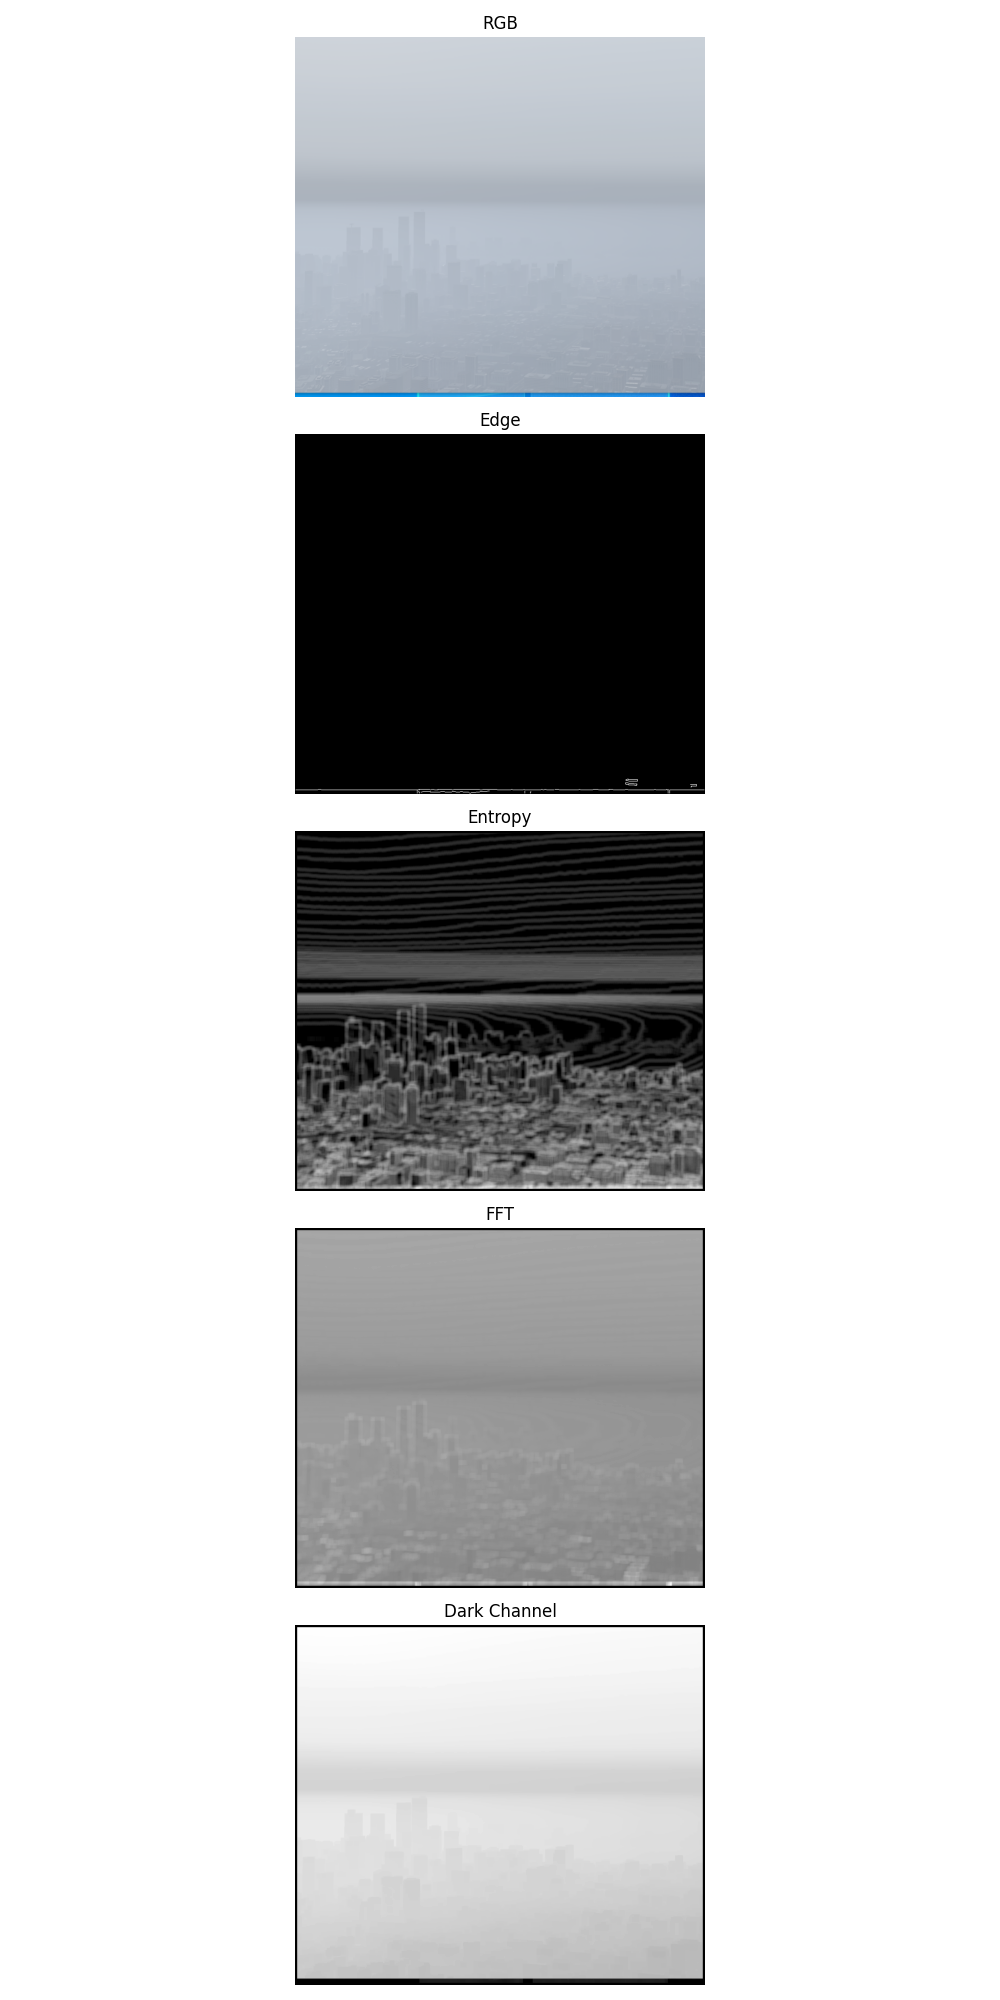
\includegraphics[width=\textwidth, trim={7.5cm 0 7.5cm 0},clip]{imgs/examples/exp_0_featuresMiles_1.8951868467819106_featuresM_3050_features.png}
      \caption{(1, 3] miles}
      \label{subfig:bin2}
    \end{subfigure}
    \begin{subfigure}[b]{0.15\textwidth}
      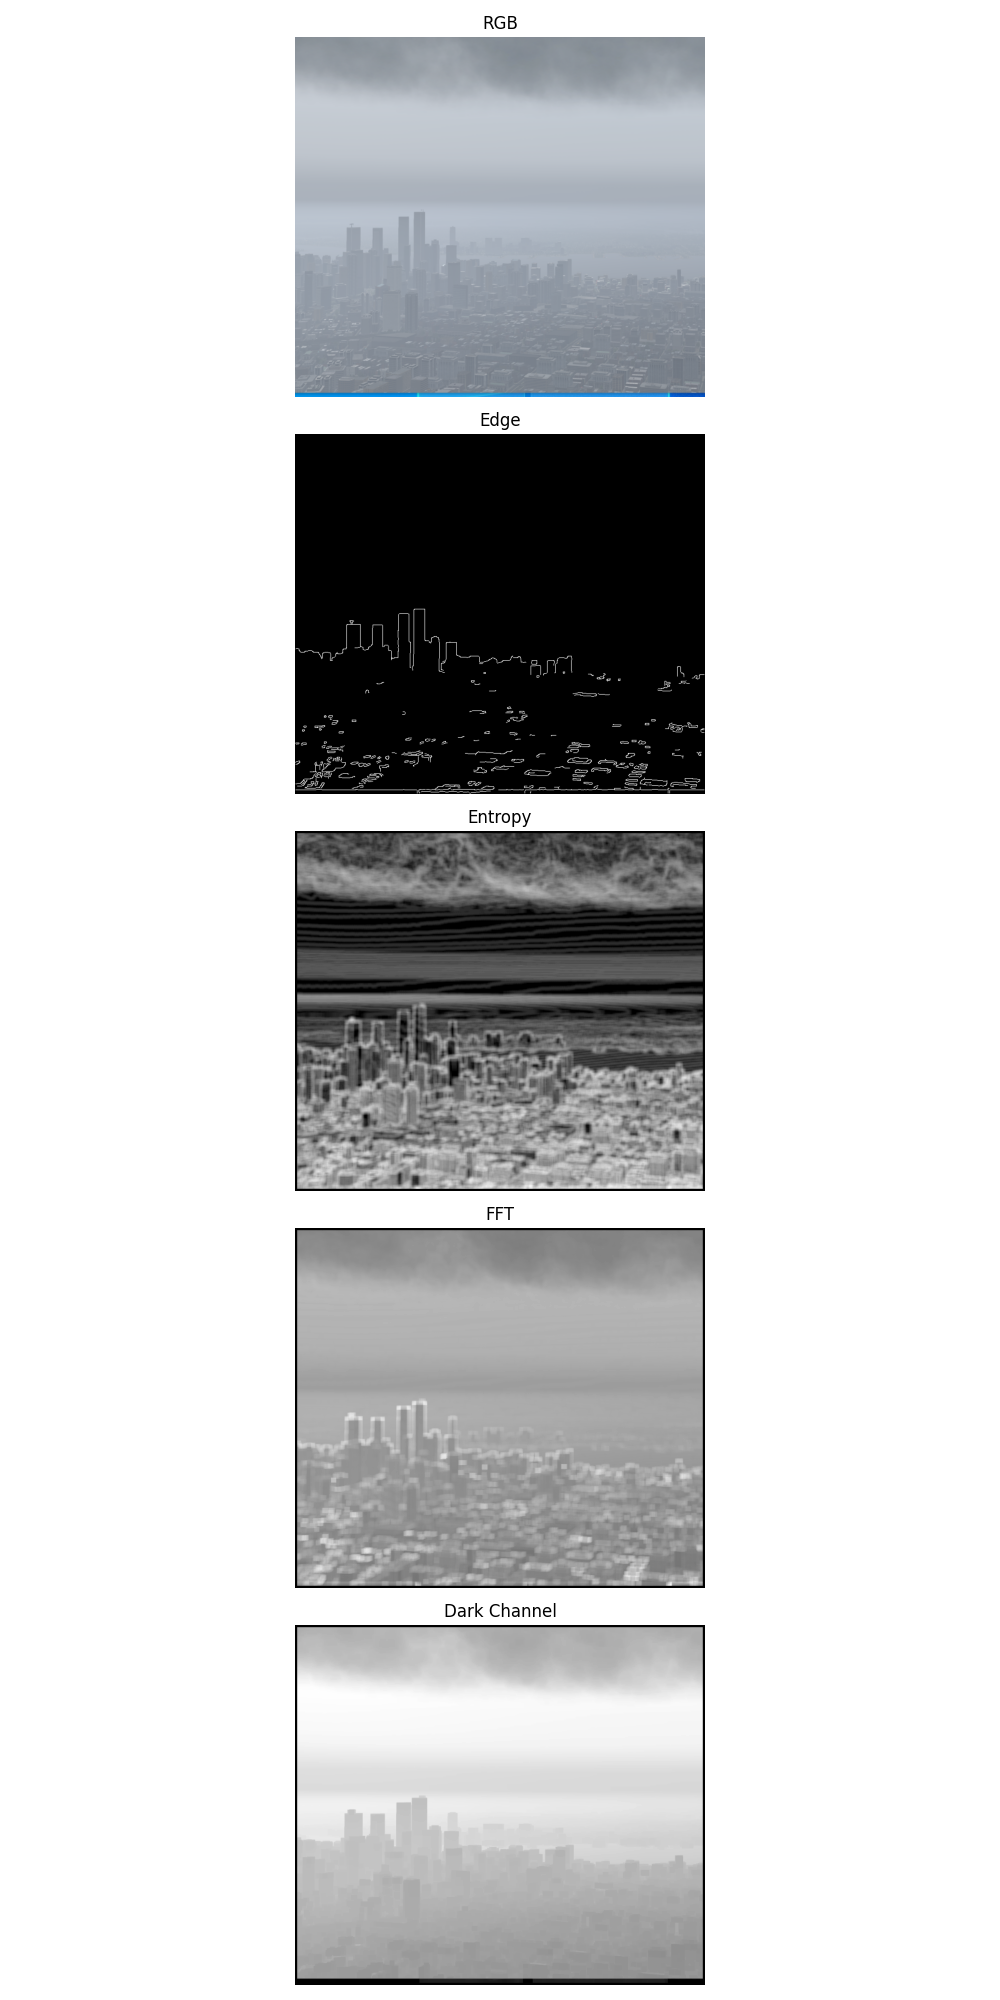
\includegraphics[width=\textwidth, trim={7.5cm 0 7.5cm 0},clip]{imgs/examples/exp_0_featuresMiles_4.038922788223744_featuresM_6500_features.png}
      \caption{(3, 5] miles}
      \label{subfig:bin3}
    \end{subfigure}
    \begin{subfigure}[b]{0.15\textwidth}
      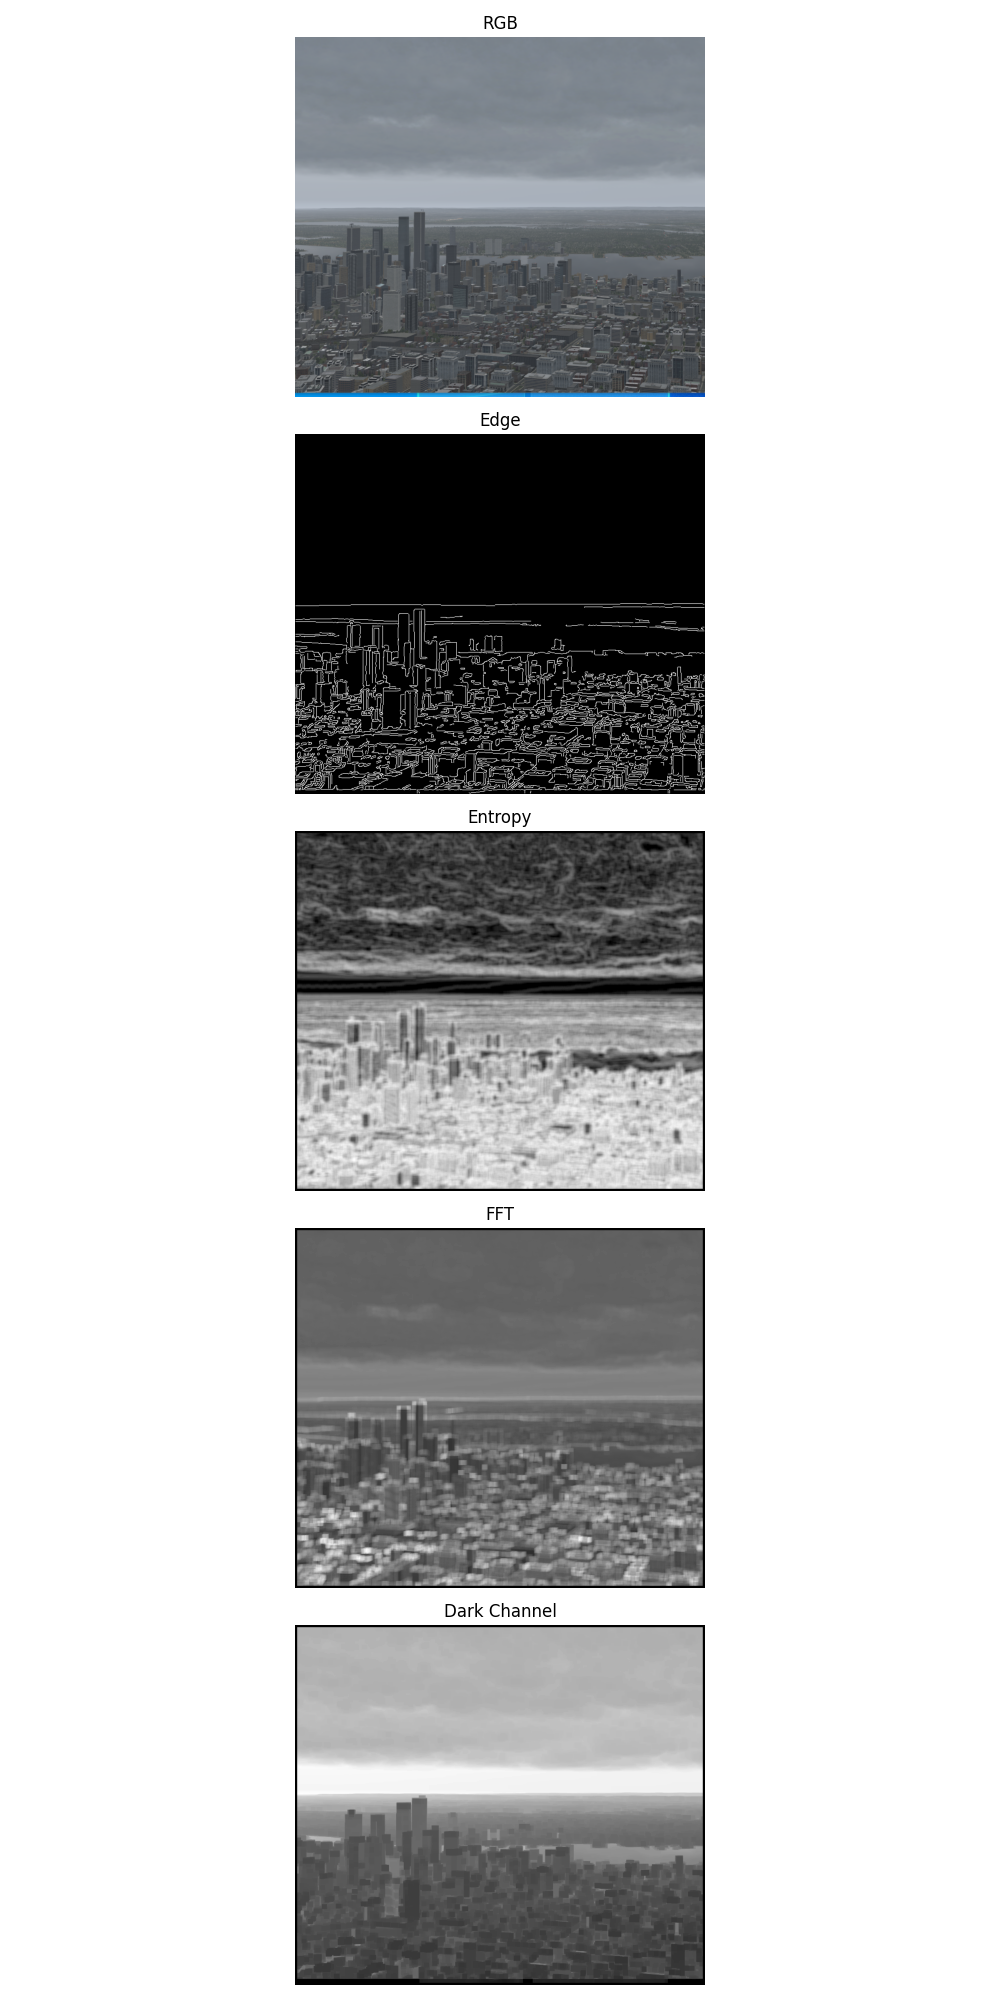
\includegraphics[width=\textwidth, trim={7.5cm 0 7.5cm 0},clip]{imgs/examples/exp_0_featuresMiles_46.1462462872979_featuresM_74265_features.png}
      \caption{> 5 miles}
      \label{subfig:bin4}
    \end{subfigure}
  
  \caption{The impact of visibility on the multiple modalities for the 6N7 Sealane 01 View. Each row shows one modality: RGB, edge map, entropy map, FFT magnitude, and dark channel prior. Each column refers to a visibility bin.}
  \label{fig:impact_vis_deg_features}
\end{figure}


\begin{table}[htbp]
\centering
\caption{Visibility Categories and Images Count}
\label{tab:vis_img_count}
\begin{tabular}{@{}lllr@{}}
\toprule
Category & Visibility in miles  & Visibility in meters & Count  \\
\midrule
4        & $\geq$ 5 miles             &     $\geq$ 8046.72m                 & 67002  \\
3        & 3 to 5 miles         &      4828.03m to  8046.72m        & 19584  \\
2        & 1 to 3 miles         &            1609.34m to 4828.03m         & 19648  \\
1        & 0.5 to 1 mile  &               804.672m to 1609.34m      & 4928  \\
0        & $\leq$ 0.5 mile   &     $\leq$ 804.672m                 & 4938  \\
\midrule
Total    &    &                      &  116100  \\
\bottomrule
\end{tabular}
\end{table}


\subsubsection{Modalities}
\label{modalities}

\textbf{Monocular Depth Estimation:}

Monocular depth maps were extracted using the Omnidata toolkit \cite{eftekhar2021omnidata, ranftl2021vision}. This toolkit provides a scalable and comprehensive method for depth estimation, which is essential for understanding the spatial arrangement of a scene. The resulting depth maps furnish a pixel-wise measurement of distance from the viewpoint, thereby facilitating an accurate representation of the three-dimensional scene structure.

It is important to note a specific limitation of the depth estimation models employed. The training methodology for these models involves masking the sky and exclusively considering the ground for depth estimation. This may present challenges for certain images within our dataset that were captured at varying altitudes.

\textbf{Normal Surface Estimation:}

In addition to depth maps, the Omnidata toolkit was also utilized for normal surface estimation \cite{eftekhar2021omnidata}. This modality provides information regarding the orientation of surfaces within the image, which is crucial for discerning the geometric properties of the scene. In contrast to the depth estimation model, the normal surface estimator considers both sky and ground details.

\textbf{Entropy Map:}

An image entropy map is incorporated as a modality to enhance the model's sensitivity to variations in visibility, particularly under low-visibility conditions. The entropy map quantifies the amount of information, or uncertainty, present in different regions of an image.

\textbf{Edge Detection:}

Edge detection serves as another key modality, particularly well-suited for long-range visibility scenarios where the delineation of objects and scene boundaries is critical. By highlighting the contours and edges within an image, this modality aids in defining shapes and structures, thereby providing a clearer distinction between different objects and features in the scene.


\begin{figure}
    \centering
% Mean of Dark Channel Prior vs Visibility
    \begin{subfigure}[b]{0.4\textwidth}
        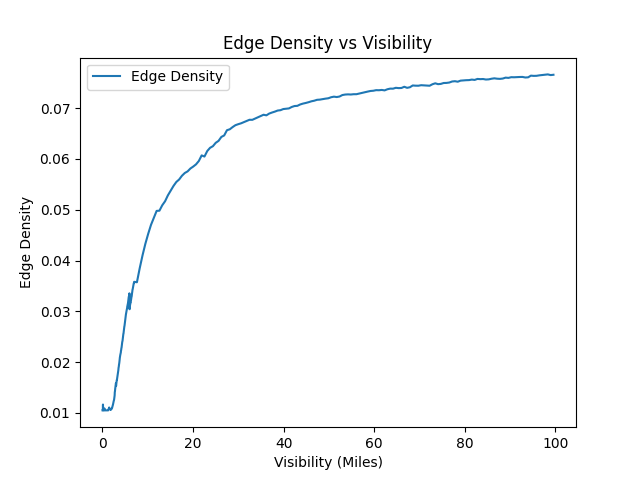
\includegraphics[width=\textwidth]{imgs/edge_density_vs_visibility.png}
    
    \end{subfigure}
    % Mean of Dark Channel Prior vs Visibility
    \begin{subfigure}[b]{0.4\textwidth}
        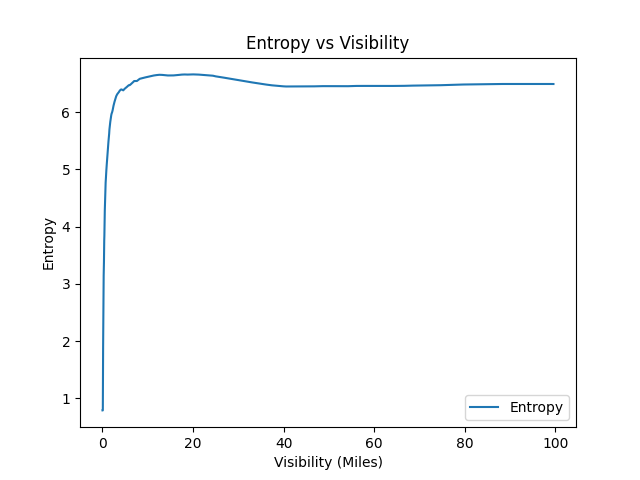
\includegraphics[width=\textwidth]{imgs/entropy_vs_visibility.png}
    \end{subfigure}
    % Mean of Edge Density vs Visibility
    \begin{subfigure}[b]{0.4\textwidth}
    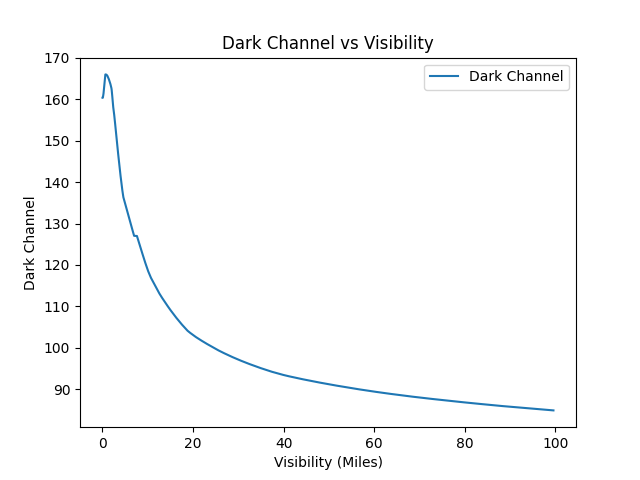
\includegraphics[width=\textwidth]{imgs/dark_channel_vs_visibility.png}
        
    \end{subfigure}
    % Mean of FFT Magnitude vs Visibility
    \begin{subfigure}[b]{0.4\textwidth}
        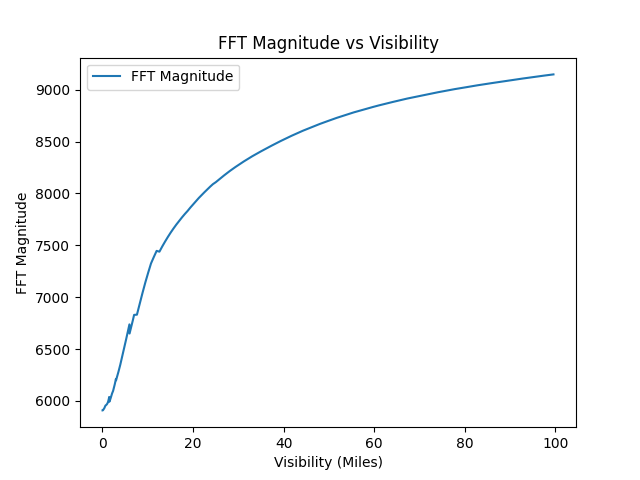
\includegraphics[width=\textwidth]{imgs/fft_magnitude_vs_visibility.png}
    \end{subfigure}
    \caption{Impact of Visibility Degradation on Edge Density (a), Entropy map (b), Dark Channel Prior (c), and FFT Magnitude (d) vs Visibility in Miles}
    \label{fig:mean_of_features}
\end{figure}

 In Figures~\ref{fig:impact_vis_deg_features} and \ref{fig:mean_of_features}, we illustrate the impact of visibility degradation on various modalities for the same scene. Each row displays a single modality, while each column corresponds to a specific visibility bin.

\subsection{Fusing Modalities}

In the literature, numerous methods have been proposed for the fusion of different modalities within multi-stream networks \cite{akkus2023multimodal, radford2021learning, jia2021scaling}. These methods range from the simple concatenation of input streams in the input space to more complex fusion strategies at various levels of the model architecture.

Early fusion \cite{huang_fusion_2020} involves concatenating or otherwise preprocessing all input streams in the input space. The combined data is then fed into a single feature extractor. While this method is the simplest to implement, it is often limited, as the feature extractor may learn to disregard some modalities, with the feature representation being dominated by a single modality.

Intermediate fusion \cite{huang_fusion_2020}, a widely adopted approach, involves feeding the different modalities into separate encoder layers before fusing the extracted embeddings. In this paradigm, the model learns to extract salient features from each modality before they are combined, thereby preventing any single modality from dominating the feature space. A significant advantage of this architecture is its compatibility with recent advancements in representation learning, such as contrastive learning or unsupervised representation learning, where fusion occurs between the encoder and decoder layers or at the initial stages of processing.

Late fusion \cite{huang_fusion_2020} represents another fusion strategy, wherein each modality is passed through its own complete network until the decision layer (e.g., a classifier). Fusion is then performed at the decision level, either through a voting mechanism between the different models or by averaging their respective outputs.

\subsubsection{Multimodal Fusion Methods}

Various techniques for multimodal fusion have been proposed in the literature, including Tensor Fusion \cite{zadeh2017tensorfusionnetworkmultimodal}, Low-Rank Fusion \cite{liu2018efficientlowrankmultimodalfusion}, and attention mechanisms \cite{NEURIPS2021_76ba9f56}. Although each method possesses its own set of advantages and disadvantages, self-attention has emerged as a foundational component for many recent large-scale models. While it typically requires a larger volume of training data, its computational cost is significantly lower compared to methods such as tensor fusion.

\subsubsection{The SeeNN Multimodal Fusion Framework}

\label{subsub:proposed}


\begin{figure}
    \centering
    \begin{subfigure}[b]{0.64\textwidth}
        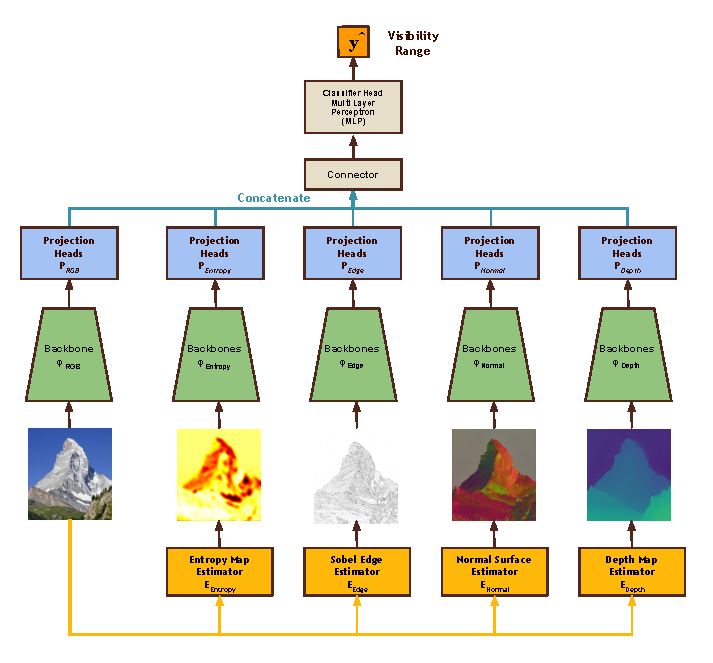
\includegraphics[width=\textwidth]{imgs/SeeNN_Expanded.pdf}
    \caption{}
    \end{subfigure}
    \begin{subfigure}[b]{0.2\textwidth}
        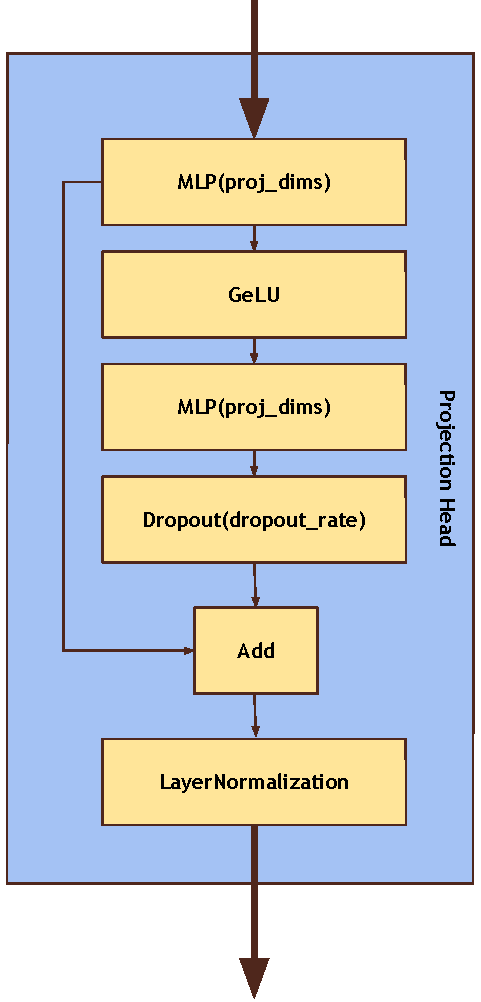
\includegraphics[width=\textwidth]{imgs/Projection Head.pdf}
    \label{fig:projection_head}
        \caption{}
    \end{subfigure}
\caption{
(a) SeeNN Framework: The framework first extracts features (entropy map, surface normals map, edge map, depth map) from the input image. Separate encoders $\phi_{m}(\cdot)$ ($\phi_{m}(\cdot)$ denotes modality encoders) process these features followed by a projection head (b), followed by fusion of these features through a Connector and prediction via a classifier $\mathbf{\hat{y}}$.
(b) Projection Head: The input vector is transformed by an MLP (Multi-Layer Perceptron) with a non-linear activation function (GeLU) and dropout for regularization.
}
\label{fig:seeeNN}
\end{figure}

The proposed SeeNN framework, illustrated in Figure~\ref{fig:seeeNN}, integrates multimodal deep learning techniques to process images concurrently with multiple derived modalities.

Initially, each input RGB image \( I \) undergoes a series of transformations via modality estimators to generate a depth map \( E_d(I) \), a normal surface map \( E_n(I) \), an edge detection map \( E_e(I) \), and an entropy map \( E_s(I) \). Each of these modalities captures distinct characteristics of the input, providing a diverse set of perspectives on the image's content.

Let $m$ denote a specific modality (i.e., generated depth map $depth$, normal surface $normal$, entropy map $entropy$, edge map $edge$, and RGB image $rgb$). We employ different backbone models $\Phi_{m}(\cdot)$ for each modality input $X_m$. In this work, we utilize DenseNet121 \cite{huang_densely_2018} as the architecture for all $\Phi_{m}$. The resulting embedding from each encoder is fed to a projection head $P_m$, which consists of a Multi-Layer Perceptron (MLP) with a non-linear activation function (GeLU) and dropout for regularization. This is followed by a layer normalization step, which is crucial for aligning the feature representations and mitigating the risk of dominance by any single modality. This process yields a feature vector \( F_m \).

This procedure is applied to the RGB image $X_{rgb}$, depth map \( X_{depth} \), normal surface map \( X_{normal} \), entropy map \( X_{entropy} \), and edge map \( X_{edge} \) to obtain the feature vectors $F_{rgb}$, $F_{depth}$, $F_{normal}$, $F_{entropy}$, and $F_{edge}$, respectively.

Following the projection heads, the SeeNN framework concatenates these embeddings into a single, comprehensive feature vector \( F \). This concatenation is represented as \( F = [F_{rgb}, F_{depth}; F_{normal}; F_{entropy}; F_{edge}] \). This composite vector is then fed to a connector module, $C$, which is responsible for fusing these modalities.

Finally, an MLP classifier head is applied to the fused feature vector to obtain the final prediction, $\hat{y}$.

For the connector module, we explored two primary methods. The first method involves passing the flattened feature vector \( F \) directly to the MLP, representing a simple yet effective fusion of the different features. The second method utilizes an attention block to perform self-attention on \( F \), followed by flattening the output and feeding it to the MLP head.

\subsubsection{Experimental Setup}

For this study, we utilized our custom-collected dataset, SeeSet V1 (\ref{sec:seeset}), which comprises 320 distinct views collected across 20 locations with varying land covers, each with visibility ranging from 0 to 100 miles. The dataset was partitioned into training and validation subsets using a holdout approach. Specifically, all views from a predefined set of locations were reserved for the validation set, ensuring that the model does not overfit to specific sceneries and instead learns to estimate visibility based on image degradation \cite{Bouhsine2022}. This resulted in a training set of $100,350$ instances and a validation set of $15,750$ instances. All images in the dataset were preprocessed to an input resolution of $224 \times 224$ pixels.

We employed the Omnidata models to preprocess the RGB images and extract the estimated Depth Map and Normal Surface \cite{eftekhar2021omnidata}. This approach, based on the DPT-Hybrid architecture \cite{ranftl2021vision}, is analogous to methods used in the literature to generate pseudo-labels from RGB data for pre-training multimodal models \cite{bachmann2022multimae, wang2024largescale}.

For the other modalities, namely the edge map and the entropy map, the RGB images were processed through handcrafted estimators, as depicted in Figure~\ref{fig:seeeNN}.

All models were trained for 100 epochs using the Adam optimizer with a learning rate of $0.001$. A batch size of $32$ was used for all training procedures.
